\item[(b)]
\section*{Task (b)}

\subsection*{Problem Statement}
Sample the analog signal \( x(t) \) with sampling frequencies \( f_{s1} = 9 \, \text{kHz} \) and \( f_{s2} = 14 \, \text{kHz} \), which yield \( x_1[n] \) and \( x_2[n] \), respectively. Sketch the corresponding DTFT spectra.

\subsection*{Theoretical Background}
Sampling an analog signal at a frequency \( f_s \) converts it into a discrete-time signal. The discrete-time Fourier transform (DTFT) of a discrete signal \( x[n] \) is given by:
\[ X(e^{j\omega}) = \sum_{n=-\infty}^{\infty} x[n] e^{-j\omega n} \]

The DTFT spectrum of a sampled signal will repeat periodically with a period of \( 2\pi \), corresponding to the sampling frequency.

\subsection*{Mathematical Derivation}
Given the analog signal:
\[ x(t) = 1 + 0.5 \cos \left(2 \pi f_{1} t \right) + 2 \sin \left(2 \pi f_{2} t \right) + \sin \left(2 \pi f_{3} t \right) \]
with \( f_{1} = 2 \, \text{kHz} \), \( f_{2} = 4 \, \text{kHz} \), and \( f_{3} = 6 \, \text{kHz} \),

1. **Sampling at \( f_{s1} = 9 \, \text{kHz} \):**
   - The discrete-time signal \( x_1[n] \) is obtained by sampling \( x(t) \) at \( t = nT_1 \) where \( T_1 = \frac{1}{f_{s1}} \).

2. **Sampling at \( f_{s2} = 14 \, \text{kHz} \):**
   - The discrete-time signal \( x_2[n] \) is obtained by sampling \( x(t) \) at \( t = nT_2 \) where \( T_2 = \frac{1}{f_{s2}} \).

\subsection*{Python Implementation and Plot}
The plot Figure~\ref{fig:ex1_b_dtft_x1} below illustrates the DTFT of \( x_1[n] \) sampled at 9 kHz, and Figure~\ref{fig:ex1_b_dtft_x2} shows the DTFT of \( x_2[n] \) sampled at 14 kHz:

\begin{figure}[h]
    \centering
    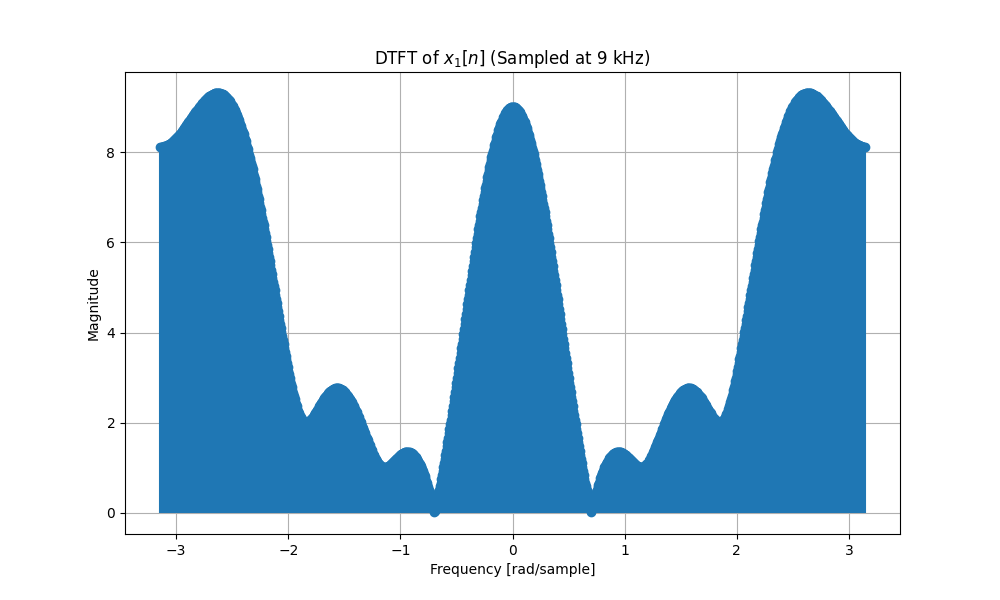
\includegraphics[width=0.8\textwidth]{fig/ex1_b_dtft_x1.png}
    \caption{DTFT of $x_1[n]$ (Sampled at 9 kHz)}
    \label{fig:ex1_b_dtft_x1}
\end{figure}

\begin{figure}[h]
    \centering
    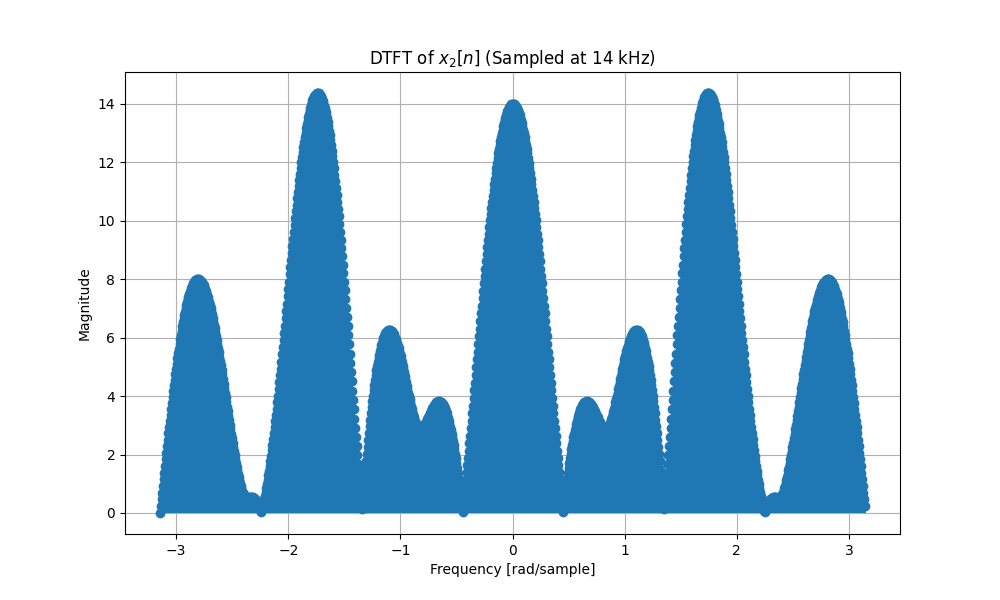
\includegraphics[width=0.8\textwidth]{fig/ex1_b_dtft_x2.png}
    \caption{DTFT of $x_2[n]$ (Sampled at 14 kHz)}
    \label{fig:ex1_b_dtft_x2}
\end{figure}

\subsection*{Conclusion}
The DTFT spectra of the sampled signals \( x_1[n] \) and \( x_2[n] \) show the frequency components of the original analog
